\documentclass[12pt]{article}
\usepackage[utf8]{inputenc}

\usepackage{graphicx}
\graphicspath{{images/}}

\usepackage{palatino}
\fontfamily{ppl}\selectfont

\title{\textbf{A Semantic Loss Function for Deep Learning with Symbolic Knowledge}}
\author{\textbf{Xu, Zhang, Friedman, Liang, Van den Broeck}}
\date{Aviral Janveja\\ Universit\"{a}t Paderborn}

\begin{document}

\maketitle

\begin{abstract}
This report investigates the paper as mentioned in the title $^1$, along with the supplementary material $^2$ provided by the authors. The paper explores the problem of deep learning methods facing difficulty in learning structured targets such as optimal paths in a graph or ranking of preferences. The authors develop a unique methodology to tackle the above issue that applies symbolic logic to deep learning. As a result, near state of the art results have been obtained along with significant improvements in predicting structured objects such as paths and rankings. The style of presentation is that of an introductory chapter for a machine learning textbook. Thus written in a self contained manner with an elaborate introduction that builds to the topic of interest in a step by step fashion. 
\end{abstract}

\section{Introduction}

\subsection{Artificial Intelligence and its Approaches}
Artificial Intelligence is a wide and interdisciplinary field that brings together many disciplines like mathematics, computer science, philosophy, cognitive sciences and more. The goal of AI research is to tackle problems of planning, reasoning, learning, perception, knowledge representation with the long term goal of achieving a state of general intelligence$^7$.\\   
Although the concept of artificial beings and intelligent mechanical objects has existed in our culture since antiquity, the solid foundation for the the field was laid down by the likes of Alan Turing, followed by Marvin Minsky, John McCarthy, Allen Newell during early and mid 20th century.\\
Since then we have seen certain key approaches develop, which have guided the direction of research in the field. Let us continue to discuss two fundamental approaches to AI, which have really shaped the field since 20th century.

\subsubsection{Symbolic AI}
Symbolic artificial intelligence is the collective term used for methods based on symbolic representation of problems and instructions based on logic and search. This was the dominant paradigm that guided research in the field of AI during 1950-1990. Experts in the field believe that continuing research in this domain will be crucial in accomplishing the long term goal of general intelligence. 
\subsubsection{Machine Learning}
This is an approach based on learning from data\begin{math}^3\end{math}, where we normally use huge amounts of data and computational resources to enable the machine to figure out an underlying pattern from a set of observations that \textit{generalize} outside the given set of example-data. Although progress has been taking place since the late 20th century, In recent times(2015-Today), this approach has really come to the fore-front and transformed the face of the computing industry.

\subsection{Combing the Two Approaches}

\subsubsection{Why Combine?}
There are certain problems which are extremely hard to learn because of their ``structured" nature.\\ 
Structured prediction\begin{math}^4\end{math} involves predicting structured objects rather than discrete, scalar or real values. The inter-relatedness between the predicted variables makes this process often infeasible with regular methods.\\ 
For instance, imagine predicting a path between a source-destination pair in a graph. It is not enough to get the individual edges between any two nodes right, rather and more importantly the overall path between the source and destination should make sense and ideally, be optimal.\\   
Therefore, in order to tackle the above problem, this paper\begin{math}^1\end{math}, aims to combine symbolic knowledge with deep learning in a unique fashion. 

\subsubsection{Current Approaches}
Most approaches that are looking to combine deep learning and symbolic knowledge, try to learn symbolic reasoning directly via a neural network.\\
This methodology is motivated by the need to have \textit{smooth differentiable models}(as adding symbolic reasoning code to a deep learning pipeline breaks this property). Although there is another crucial property that is desirable here, \textit{preserving the logical meaning} of the symbolic knowledge. Unfortunately, while making reasoning differentiable, the precise logical meaning of the knowledge is often lost in the above approaches. For example, you can try learning the paths in a graph via a neural network, but the logical meaning behind ``whether the path is valid ?" is not considered by the neural network in any way.\\
So, as a recap it is to be noted that the following two properties are crucial for us - 
\begin{itemize}
    \item Differentiability of the model.
    \item Preserving the Semantic meaning of the symbolic knowledge.
\end{itemize}

\subsubsection{A Unique Approach}
In order to tackle the problem of differentiable, yet sound logical reasoning, a distinct approach has been presented. From first principles(which are a set of intuitive axioms), a differentiable \textit{semantic loss} function is developed for the neural network.\\
To understand what we mean, let us take an example. Let us say that the neural network might output several paths for a path predicting task on a given graph. But we require only those paths that are meaningful and legal. This ``meaningfulness" of a valid path is the symbolic knowledge that we have. Further, we are adding this symbolic knowledge to our learner (the neural network) in the form of a ``logical constraint".\\ 
This constraint is the additional logical condition that has been applied to the output of the neural network in order to capture the symbolic knowledge connecting the different outputs - \\ 
\begin{itemize}
    \item The semantic loss function precisely captures the meaning of that constraint, and is independent of its syntax.
    \item The semantic loss measures how well the outputs of a neural network match a given constraint.
\end{itemize}

\subsection{Further Ahead}
After having arrived at the idea of a ``semantic loss function" that captures both the crucial properties mentioned above - ``Differentiability" and ``Preserving Semantic meaning". We can start exploring the semantic loss and its integration into the learning model.\\
In order to do that, let us first briefly build from a fundamental concept that is pre-requisite here - Propositional Logic.

\begin{figure}[htp]
    \centering
    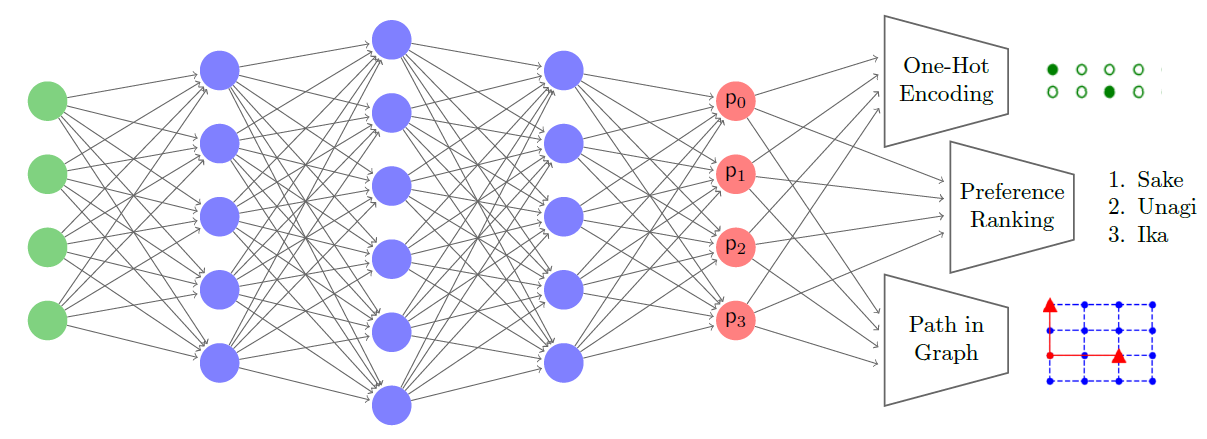
\includegraphics[width=12cm, height=4cm]{image1}
    \caption{Neural network output being fed into the semantic loss functions for different constraints.$^1$}
    \label{image1}
\end{figure}


\section{Propositional Logic}

In order to define semantic loss formally, we make use of concepts in propositional logic$^5$. Propositional logic is also known as Statement logic or sometimes zeroth-order logic. 
\begin{itemize}
    \item Atomic propositions are logical sentences without connectives which can be either true or false. They are described here as boolean variables denoted by upper-case letters X,Y and so on.
    \item Sets of variables are written in bold upper-case, \textbf{X,Y} and so on.
    \item Compound propositions can be formed by connecting atomic propositions via connectives such as AND($\wedge$), OR($\vee$) and NOT($\neg$).
    \item Compound logical sentences or propositions which can either be true or false. Here we denote them using $\alpha, \beta$ and so on. They are also called a \textit{formula} or a \textit{constraint}.
    \item A particular \textit{state or valuation} is denoted by lower-case letters x,y and so on. A state is an instantiation (true/false, 0/1) to all variables(atomic propositions) in a compound proposition or in a set of variables. 
\end{itemize}

Now, There are 3 types of propositions - 
\begin{enumerate}
    \item Valid proposition: When a compound proposition is true for all possible valuations. A trivial example of a valid sentence is $P \vee\neg P$. It is always true, hence also called a tautology.
    \item Satisfiable proposition: It is true for some (at least one) evaluation.
    \item Unsatisfiable proposition: It is not true for any evaluation. for instance, $P \wedge\neg P$.
\end{enumerate}

Another important concept that is crucial for us is that of \textit{entailment}. 
\begin{itemize}
    \item A state x satisfies $\alpha$, denoted as ``$x\models\alpha$" when the sentence  $\alpha$ evaluates to be true in that state/valuation.
    \item A sentence $\alpha$ entails $\beta$, denoted as ``$\alpha\models\beta$" when for every valuation/state that makes $\alpha$ true, $\beta$ is also true.(all valuations that satisfy $\alpha$ also satisfy $\beta$). 
    \item A sentence $\alpha$ is logically equivalent to $\beta$, denoted as $\alpha\equiv\beta$ when both $\alpha\models\beta$ and $\beta\models\alpha$.
\end{itemize}
The neural network's output row vector is denoted as p. The values in p represent the probability of an output, these probabilities fall in the range [0,1]. 
Figure \ref{image1} shows us three different possible output constraints(propositions). These have varying difficulty and have been studied in out experiments. 
Firstly, we examine the exactly one constraint that captures the encoding used in multi-class classification. It states that from a set of indicator variables $(X_1, X_2, ...X_n)$, exactly one must be true. 
This is enforced through a logical constraint(proposition) $\alpha$ by conjoining sentences of the form - 
\begin{itemize}
    \item $\neg X_1 \vee \neg X_2\ $ for all variable pairs.(at most one variable is true)
    \item $X_1\vee X_2...\vee X_n$.(at least one variable is true)
\end{itemize}


\section{The Semantic Loss$^1$}
Having had a basic idea of about propositional logic, In this section, The semantic loss will be defined along with the intuition behind the idea.\\
The semantic loss function $L^s(\alpha,p)$ is a function of a proposition $\alpha$ in propositional logic, defined over variables \{$X_1, X_2,...,X_n$\} and a vector of probabilities p for the same variables. The element $p_i$ corresponds to a single output of the neural net and denotes the predicted probability of variable $X_i$.\\
Looking at it once again. The semantic loss between the exactly one constraint from the previous section and the neural net output vector p, is intended to capture how close the prediction p is to having \textit{exactly one output($P_i$) set to true(1) and all others to false(0)}, regardless of which output is the correct one.\\
The \textit{definition} is as follows - \\ 
Let p be a vector of probabilities, one for each variable \{$X_1, X_2,...X_n$\} and let $\alpha$ be a proposition over those variables. The semantic loss between $\alpha$ and p is given by -
\begin{displaymath}
L^s(\alpha,p) \propto -\ log \ \sum_{x\models\alpha} \ \prod_{i:x\models Xi} p_i \\ \prod_{i:x\models\neg Xi} \ (1-p_i) \end{displaymath} 

Intuitively, for better understanding, the semantic loss is proportional to a negative logarithm of the probability of generating a state - that satisfies the constraint, when sampling values according to p.

The definition follows \textit{uniquely} from the set of intuitive axioms considered in the supplementary appendices$^2$.
The advantage in utilizing a set of axiomatic assumptions in order to imply the definition of a semantic loss function is that - if any alternative semantic loss function is proposed to enforce the logical constraints, at least one of the axioms will be violated$^6$. This will bring forth the differences in the assumptions made. The definition is also enough in itself for getting a clear picture of the experiments presented in the next section.


\section{Practical Experiments}

\begin{figure}[htp]
    \centering
    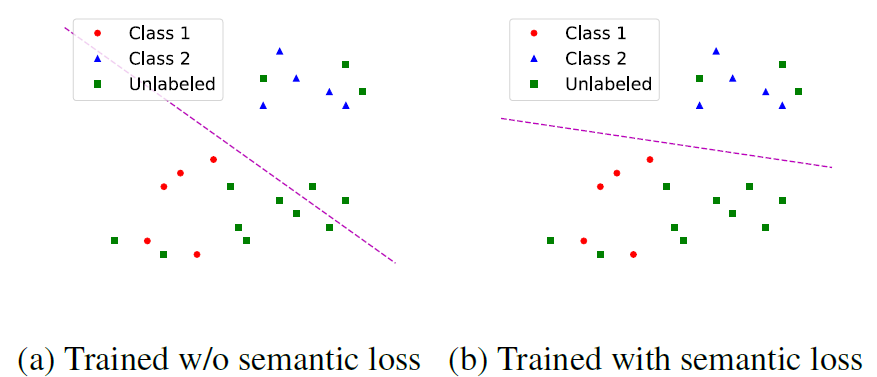
\includegraphics[width=12cm, height=5cm]{image2}
    \caption{Binary classification toy example: a linear classifier without and with semantic loss.$^1$}
    \label{image2}
\end{figure}
Many of the deep learning models take large amount of data for granted, here big data is essential for the discovery of accurate representations. In order to sustain this progress and diminish the need for more labeled data, there is growing interest in utilizing unlabelled data for augmenting the classifiers' prediction power.\\ In this section, we show how semantic loss gives significant practical improvements in semi-supervised classification and thus naturally qualifies for this role.

\subsection{Illustrative Example}
Consider the binary classification task in figure \ref{image2}. 
\begin{itemize}
    \item In 2(a), not considering the unlabeled data, the linear classifier only makes use of the data labels to learn to distinguish the two classes.
    \item However, in 2(b) the unlabeled data carries information, with respect to the property which would give them their own particular label.
    \item This is the crux of semantic loss for semi-supervised learning - a model must confidently assign a class, even to unlabeled data. This allows the model to result in a more accurate decision boundary.
\end{itemize}
\subsection{Method}
The Semantic loss, in simple words is another regularization term, that can be plugged into the existing loss function directly. Specifically, with weight w, the new combined loss is 
\begin{displaymath}
existing\ loss + w.\ semantic\ loss.
\end{displaymath}
When, output space has a simple constraint over it, the semantic loss can be calculated using Definition in section-3. For instance, In the exactly one constraint for n-class classification, the semantic loss reduces to - 
\begin{displaymath}
L^s(exactly-one,p) \propto -\ log \ \sum_{i=1}^{n} p_i\ \prod_{j=1, j\neq1}^{n} \ (1-p_j)
\end{displaymath}
where values $p_i$ denote the probability of class i as predicted by the neural net.
\subsection{Experimental Evaluation}
The simple addition to the loss function of standard deep-learning architectures yields near state of the art performance in semi-supervised classification on MNIST, FASHION, and CIFAR-10 data-sets.\\
Our final set of experiments study the benefits of semantic loss for learning tasks with highly structured output, such as preference learning and path prediction in a graph. In these scenarios, the task is two-fold: learn both the structure of the output space, and the actual classification function within that space.\\ 
By capturing the structure of the output space with logical constraints, and minimizing semantic loss for this constraint during learning, we are able to learn networks that are much more likely to correctly predict structured objects.\\
For instance, In the case of optimal graph path prediction. Although incoherent path accuracy showed no significant improvement via the semantic loss. The significant improvement in the coherent path accuracy displayed the crucial role that semantic loss played in guiding the network to jointly learn true paths, rather than optimizing each binary output individually.\\
We further see this by observing the large increase in the percentage of predictions that really are paths between the desired nodes in the graph.


\section{Conclusion \& Future Work}
In conclusion and looking forward to future progress, we can summarize as follows - 
\begin{itemize}
    \item In this presentation, the key identified challenges for deep learning such as reasoning and  and semi-supervised learning were explored.
    \item A unique way of combining propositional logic and automated reasoning with existing deep-learning architecture was demonstrated.
    \item The semantic loss provided significant benefits during semi-supervised classification and structured prediction for highly complex output spaces.
    \item As per the authors$^1$, an interesting direction for future progress is to come up with effective approximations for semantic loss function. Such approximations could be useful for settings where the methods described in the paper are not sufficient.
    \item It is also interesting to note that symbolic integration to a learning pipeline could help guard against the inherent biases in data which many a times introduce bias in the overall learning process. \item Finally, such a semantic loss is a promising step forward in the creation of \textit{hybrid} AI models that could be the key to creating generally intelligent systems in future.
\end{itemize}

\section*{References}

\begin{itemize}
    \item [1]: Jingyi Xu, Zilu Zhang, Tal Friedman, Yitao Liang, Guy Van den Broeck. A Semantic Loss Function for Deep Learning with semantic knowledge. In ICML 2018. 
    \item [2]: Supplementary Material for 1. Appendix A, B, C and D.
    \item [3]: Discussion between the authors(1) and reviewers from ICLR 2018 Conference.(openreview.net)
    \item [4]: Prof.Yaser Abu-Mostafa, Learning from Data, California Institute of Technology and Prof.Eyke Hüllermeier, Machine Learning-I, University of Paderborn.
    \item [5]: Prof. Deepak Khemani, Propositional Logic, YouTube Lecture given at the Indian Institute of Technology Madras, for NPTEL.
\end{itemize}

\end{document}
